When formulating the test case search problem as a many-objective optimisation problem, the goal is to minimize all the individual
distances from all the test targets in the class under test.


One of the most popular multi-objective algorithms for this problem is the Non-dominated Sorting Genetic Algorithm II (NSGA-II).
This algorithm is based on three principles:
\begin{itemize}
    \item It uses elitism when evolving the population: the most fit individuals are carried over along the offsprings.
    \item It uses an explicit diversity-preserving mechanism, the Crowding distance.
    \item It emphasizes the non-dominated solutions, as its name suggests.
\end{itemize}

First of all, in the context of test cases, domination can be expressed by the following relation:
\begin{figure}[htbp]
    \centering
    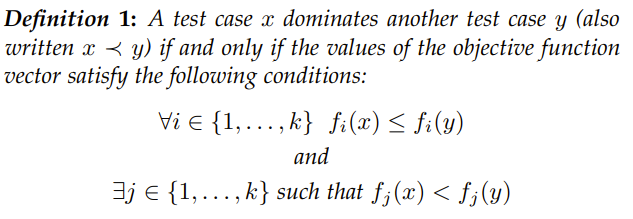
\includegraphics[scale=0.7]{./figures/test_Case_domination.PNG}
    \caption{Test case domination}
    \label{fig:test case domination}
\end{figure}


DynaMOSA, Dynamic Many-Objective Sorting Algorithm [1] is an approach that focuses on ..., and has been developed as an evolution 
of MOSA. This latter solution implements a many-objective GA to tackle test case generation and has three main features: 
\begin{itemize}
    \item instead of ranking candidates for selection based on their Pareto optimality, it uses a preference criterion.
        This criterion selects the test case with the lowest objective score for each uncovered target; these selected individuals
        are given a higher chance of survival, while other test cases are ranked with the traditional NSGA-II approach.
    \item The search is focused only on the uncovered coverage targets.
    \item All tests that satisfy one or more of the uncovered targets will be archived and used as the final test suite once the search ends.
\end{itemize}

In many-objective optimisation problems, candidate solutions are typically evaluated in terms of Pareto dominance and Pareto optimality.


DynaMOSA has been employed with Java classes.

Traditionally, with evolutionary search-based approaches, the algorithm is applied multiple times, 
once for each coverage criterion; doing so may 
Ultimately, however, the effectiveness of the solution depends on the problem